% \vspace{-0.2cm}
\section{Discussion}
\label{sec:discussion}

\begin{figure}[t]
    \centering
    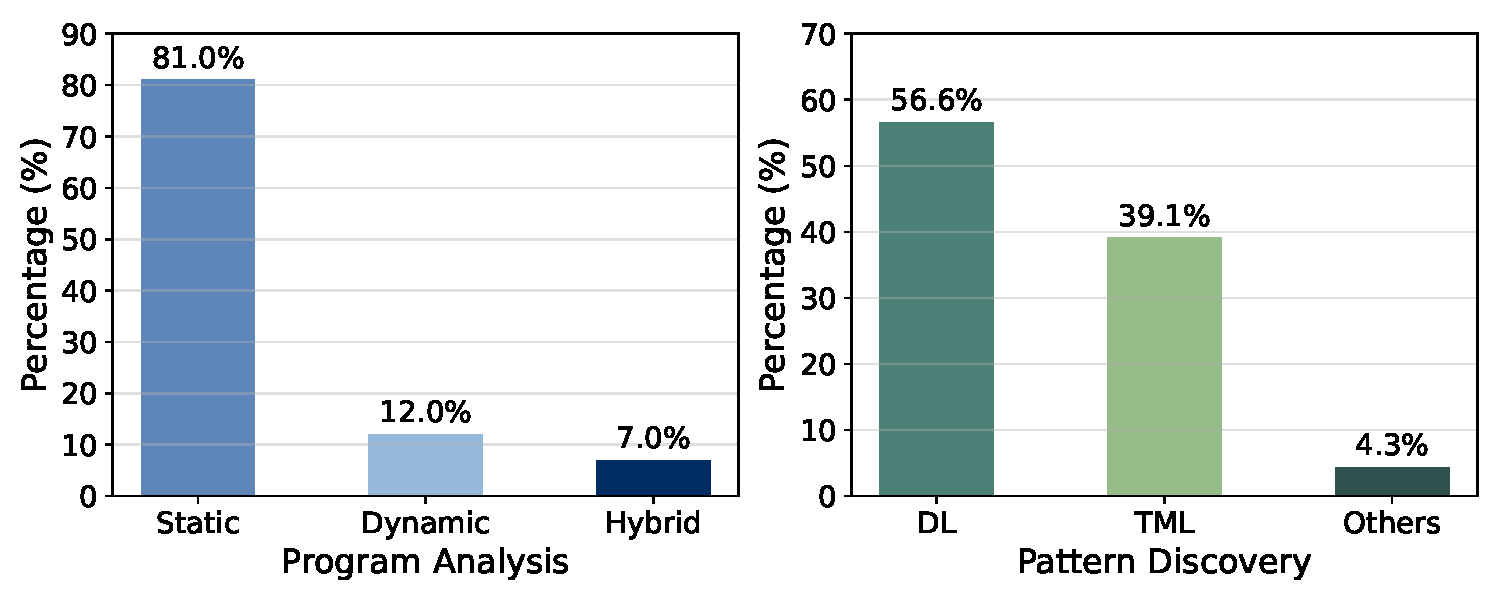
\includegraphics[width=0.76\linewidth]{fig/paper_tech.pdf}
    % \vspace{-0.1cm}
    \caption{The overall distribution of investigated approaches in Android malware detection.}
    \label{fig:paper_distribution}
    \vspace{-0.3cm}
\end{figure}

\bulletpoint{Systematic investigation}
To better understand the efforts dedicated to Android malware detection, we conduct a systematic literature review since 2011.
Aiming for the inclusion of a broad range of papers, we follow the search strategies used in~\cite{liu2022deep,liu2020review}.
Specifically, we perform searches in key digital libraries, such as the ACM Digital Library and IEEE Xplore, using specific keywords, including \texttt{android malware detection}, \texttt{android analysis}, and \texttt{android malware}.
Then, a careful screening of titles and introductions is followed to selectively exclude studies unrelated to our research topic.
This meticulous process ultimately leads to the identification of 258 related papers.

We subsequently categorize these papers based on the program analysis and pattern discovery techniques they employ.
Figure~\ref{fig:paper_distribution} shows the distribution of these techniques.
Our analysis reveals that \textit{static analysis} is the predominant technique utilized to extract features from apps, followed by \textit{dynamic} and \textit{hybrid analysis}.
For pattern discovery, \textit{machine learning}, including both traditional machine learning (TML) and deep learning (DL) models, are extensively used to identify malicious patterns.
Particularly notable is the significant increase in the utilization of static feature extraction and ML-based techniques in recent years. 
This evolving trend highlights the importance of our study, seeking to provide an in-depth understanding of the contemporary landscape in ML-based Android malware detection.

\bulletpoint{Dataset considerations}

\bulletpoint{App packing and it impact}
To protect applications from reverse engineering and tampering, many developers employ app packing techniques that obfuscate the original code structure~\cite{dong2022did,duan2018things}.
Such techniques can substantially degrade the effectiveness of static analysis-based malware detectors, as they hinder the extraction of meaningful features from packed apps.
In this study, to systematically examine the state of ML-based Android malware detection, we focus primarily on unpacked apps, which is consistent with the scope of most prior work~\cite{chen2023continuous,wu2021homdroid}.
During dataset construction, we identify an app as packed if it employs any known packing tools (\textit{e.g.,} Qihoo 360) and exclude these apps to ensure reliable static feature extraction.
We acknowledge that packing techniques can increase static feature extraction failure rates, negatively impacting the performance of static analysis-based detectors.
To mitigate this limitation in practical deployments, future detectors may benefit from integrating static and dynamic analysis techniques, enabling more robust feature extraction in the presence of packing and obfuscation.
In this work, our objective is to evaluate and understand the performance characteristics of ML-based Android malware detectors under controlled and comparable conditions.
A systematic investigation of app packing techniques and their impact on malware detection effectiveness is an important and complementary direction, which we leave for future work.

\bulletpoint{Potential of large language models in Android malware analysis}
Large Language Models (LLMs) have demonstrated remarkable capabilities in natural language processing, code understanding, and reasoning tasks.
Building upon the findings and insights from our study, we believe that LLMs hold substantial promise in the domain of Android malware analysis, particularly in the following areas:
(1) Feature space exploration: LLMs can assist in selecting and combining discriminative features to enhance the performance of malware detectors.
By analyzing the impact of different feature sets on app behavior description, LLMs can guide the construction of more effective and concise feature representations.
(2) Semantic understanding of malicious behavior: LLMs can mine high-level malicious semantics directly from code, improving the interpretability of detection systems and offering deeper insight into the behavioral mechanisms of malware.

For example, LLMs can be employed to analyze various features that describe the same malicious behavior, assess their respective impacts on detector performance, and identify the most effective feature combinations for comprehensive behavior representation.
Furthermore, LLMs can summarize the semantics of a group of functions within an application to uncover specific operations—such as sensitive information collection, data exfiltration, or command-and-control communication.
These semantic summaries can then be used to enhance the characterization and detection of potentially malicious behaviors.

\bulletpoint{Threats to validity}
\jh{There are two main threats to the validity of our study.}
First, our research mainly focuses on investigating general ML-based Android malware detectors.
That is, we do not include the methods designed to solve a particular challenge like malware evolution.
Specifically, there have been several attempts~\cite{narayanan2016adaptive,zhang2020enhancing,chen2023continuous,xu2019droidevolver} starting to mitigate the challenges we have identified.
For instance, the recent APIGraph~\cite{zhang2020enhancing} identifies semantically similar API calls to enhance detectors' robustness against malware evolution.
Integrating this strategy with popular detectors like Drebin and MamaDroid leads to 5\% - 10\% detection improvements over a one-year malware evolution.
Nevertheless, our findings still hold, as these improvements are insufficient compared to the reduction of around 30\% observed in our study.
It is our aspiration that this study can motivate more researchers to focus on these challenges and develop effective solutions to mitigate them.

Second, inconsistencies might exist between our evaluation and the reported ones due to different settings, such as datasets, metrics, and toolchains.
To mitigate experimental biases and provide a fair comparison, we design a general-purpose framework.
Specifically, we adopt standardized techniques across all tasks, including feature extraction and ML modeling.
We also incorporate many evaluation scenarios, such as training data sizes, malware evolution, and efficiency, to ensure a comprehensive measurement using our crafted dataset.
It is our hope that the framework can facilitate future work in ML-based Android malware detection.

\tosem{Disucss the dataset limitation again, and highlgiht our additional experiments again... to say our finding still hold.}